\section{User Study}
\subsection{Introduction}

To validate the usefulness of our system we decided to conduct a Within-Subjects User Study. The user study was designed to show the capacity of the system for being used in research. The study was designed to test the effectiveness of users using volumetric displays under different conditions.

\subsection{Experimental Variables}

For this study we wanted to evaluate the difference in performance of participants in interacting with volumetric screens directly with their hands vs via teleoperation. 

Our two independent variables which we varied over the study were: 
\begin{itemize}[itemsep=-0.25em]
	\item \textbf{3D Perspective}: (On/Off). This controls if the system is able to use the eye tracking system to create the illusion of a 3D volumetric display as opposed to a fixed perspective on a standard monitor as can be seen in Fig~\ref{fig:direct-vs-offset}.
	\begin{figureBox}[label={fig:direct-vs-offset}, width=0.8\linewidth]{Direct \& Offset Interaction}
		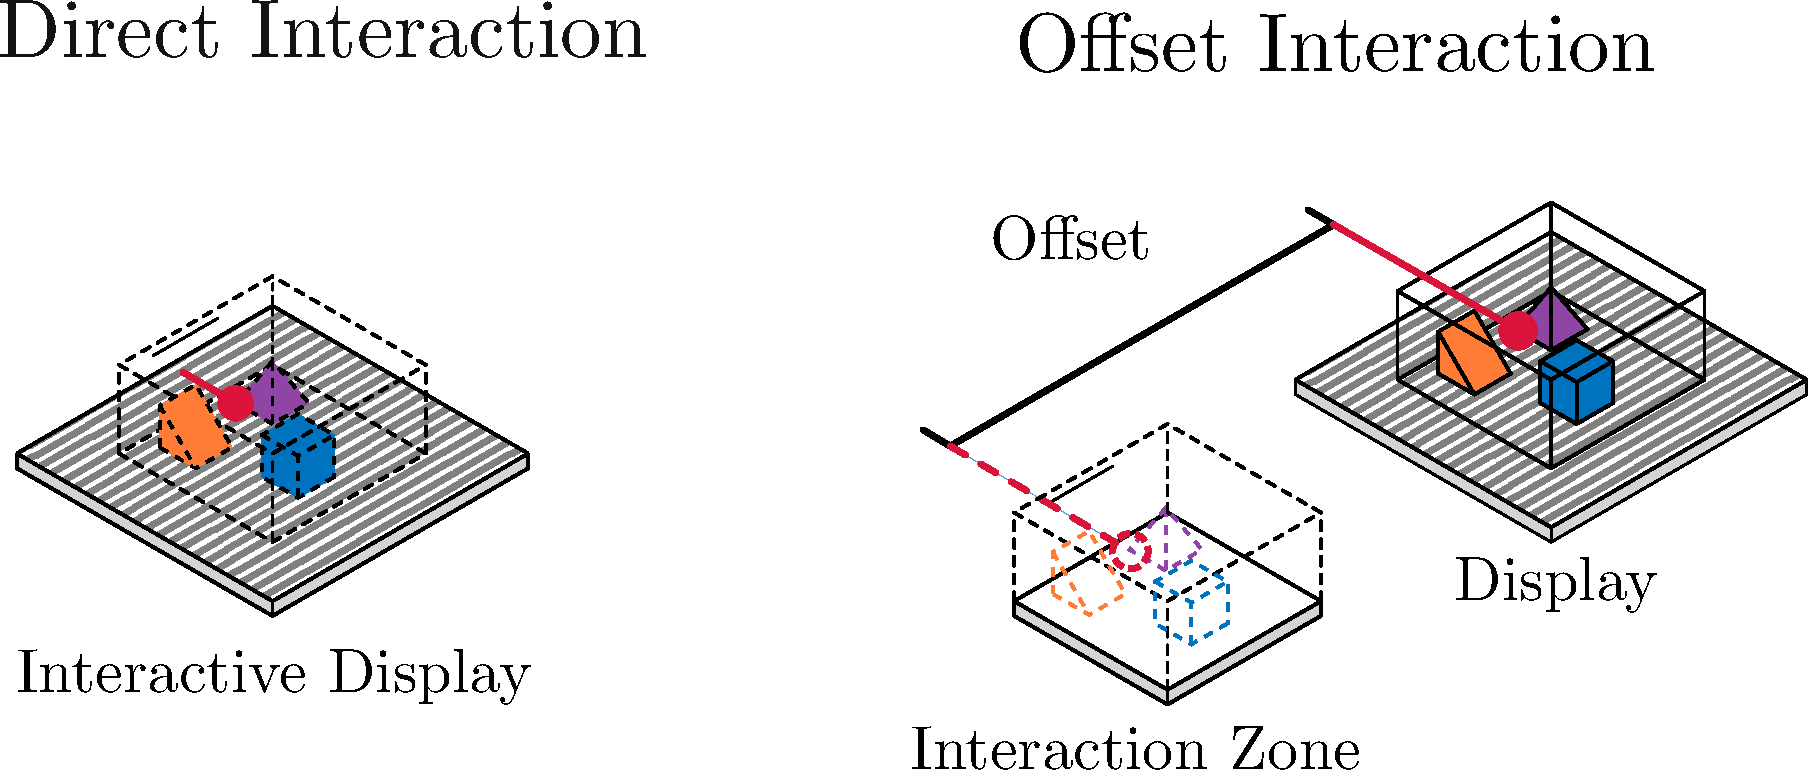
\includegraphics[width = 0.8\linewidth]{./implementation/figures/direct-vs-offset.pdf}
	\end{figureBox}
	\item \textbf{Interaction Offset}: (On/Off). This controls if display is directly in front of the participant or if it is offset by a fixed amount as can be seen in Fig~\ref{fig:2D-vs-3D}.
	\begin{figureBox}[label={fig:2D-vs-3D}, width=0.8\linewidth]{2D \& 3D}
		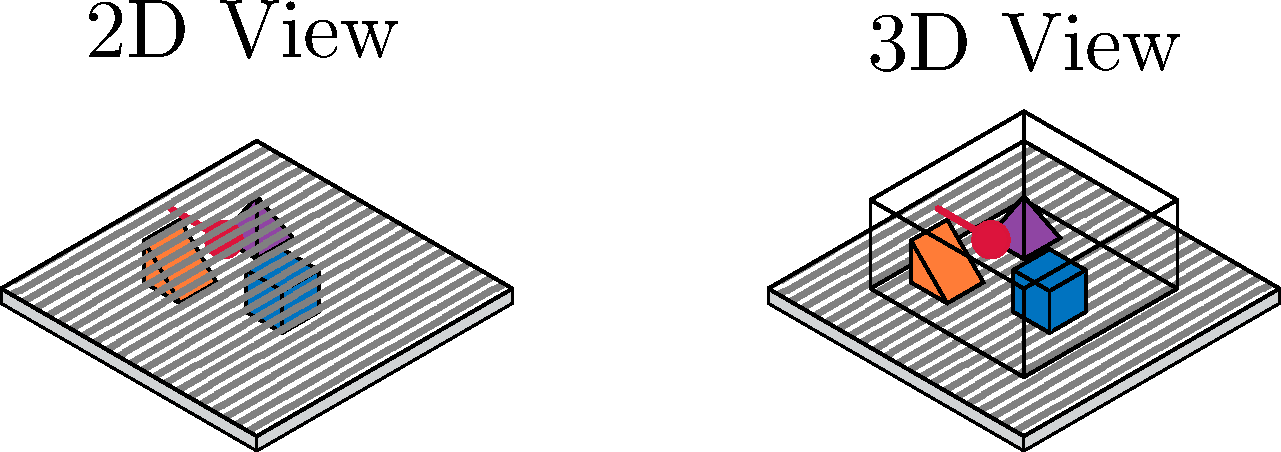
\includegraphics[width = 0.8\linewidth]{./implementation/figures/2D-vs-3D.pdf}
	\end{figureBox}
	
\end{itemize}

We made sure to control for the following variables: We made sure that the five tasks were the same in each condition. We also made sure that the position of the participant, the tracking camera, and the zone of interaction were the same in each condition as can be seen in Fig~\ref{fig:test-setup}. We were careful to ensure the lighting conditions inside the room did not change. When using an offset position we placed another display where the old display was to ensure tracking was consistent.

\begin{figureBox}[label={fig:test-setup}, width=0.8\linewidth]{Test Setup}
    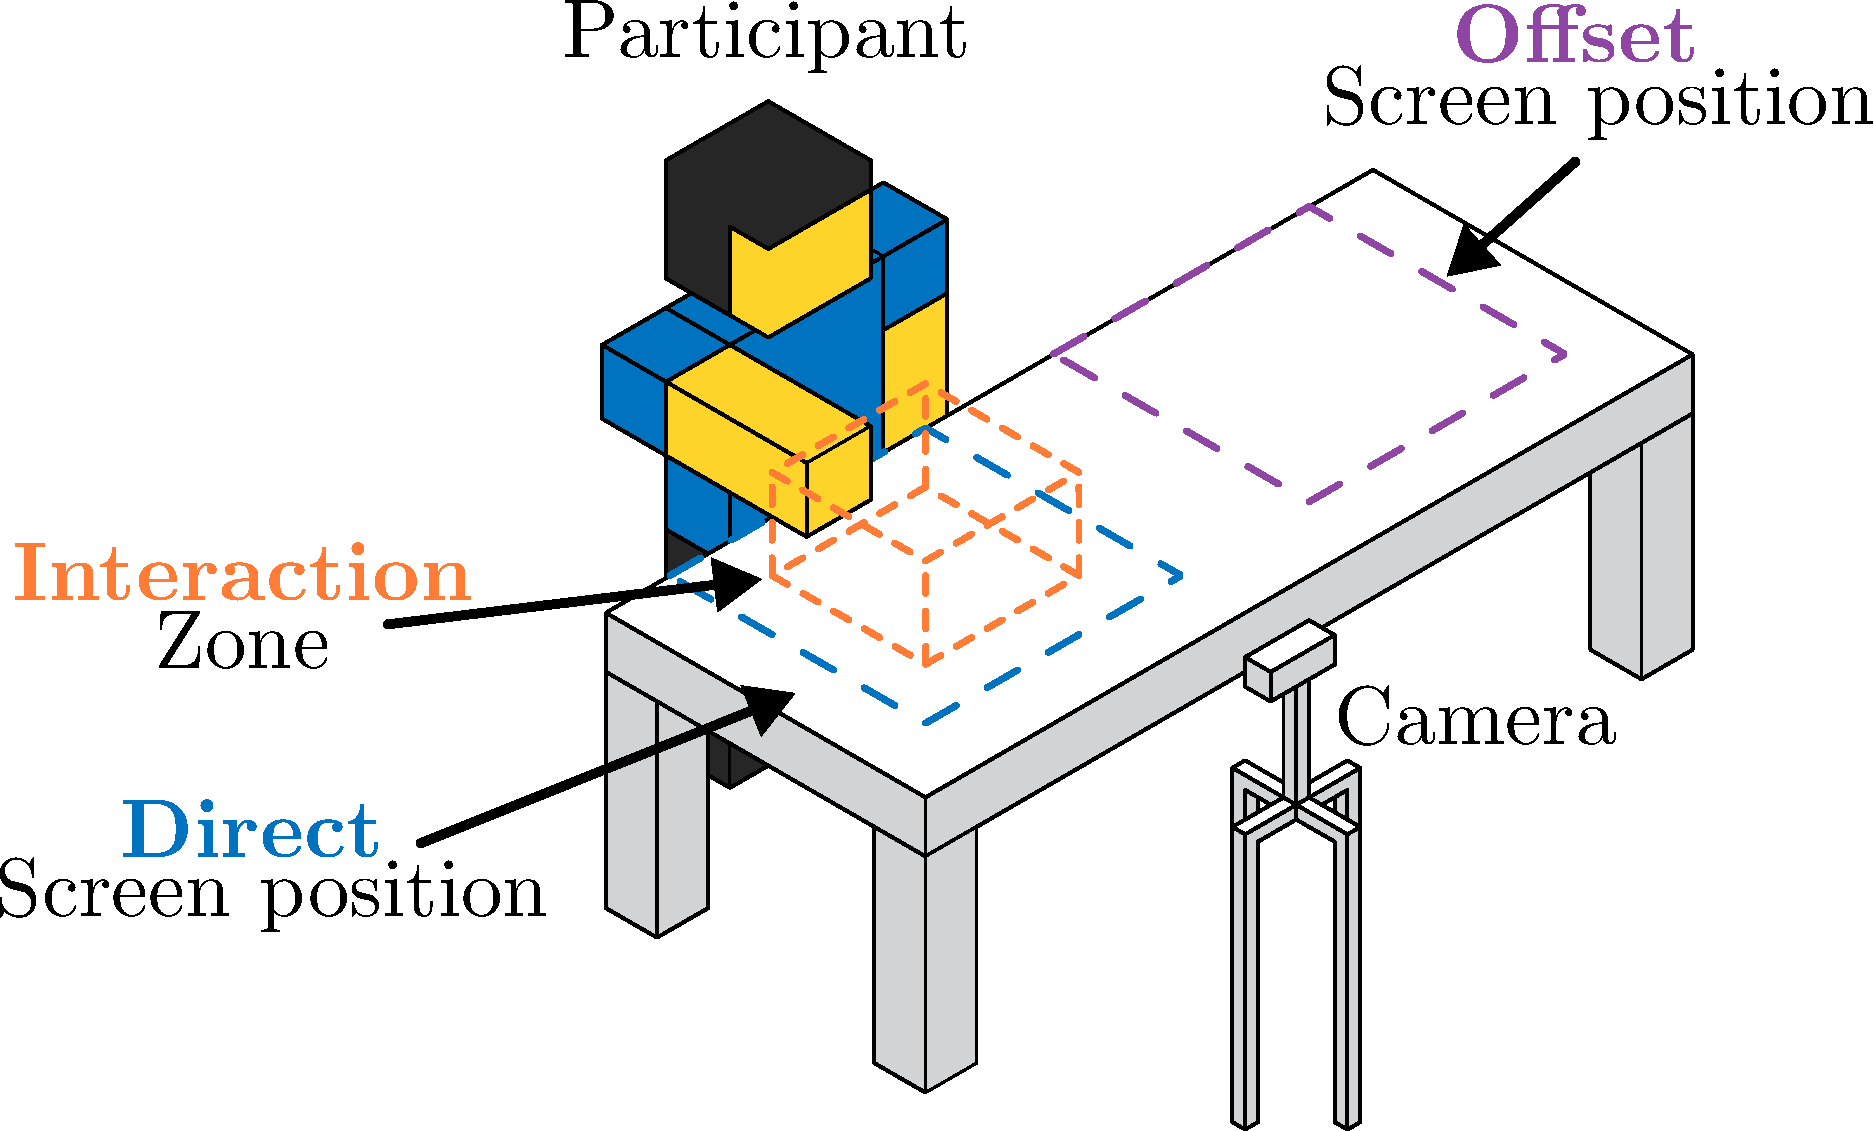
\includegraphics[width = 0.8\linewidth]{./implementation/figures/test-setup.pdf}
\end{figureBox}

\subsection{Tasks}
In each of the 4 conditions the participant must complete the same 5 tasks. The tasks are designed to be simple but more difficult to complete if not in 3D. To complete a task a participant must trace the path between the points with their index and middle finger in the order the simulator presents to them. A green point is completed segment, an orange point represents the next point to be completed and a red point in the current position of the participants hand as can be seen in Fig~\ref{fig:test-setup}. \\ 

\begin{figureBox}[label={fig:task-example}, width=0.8\linewidth]{Completing a task}
    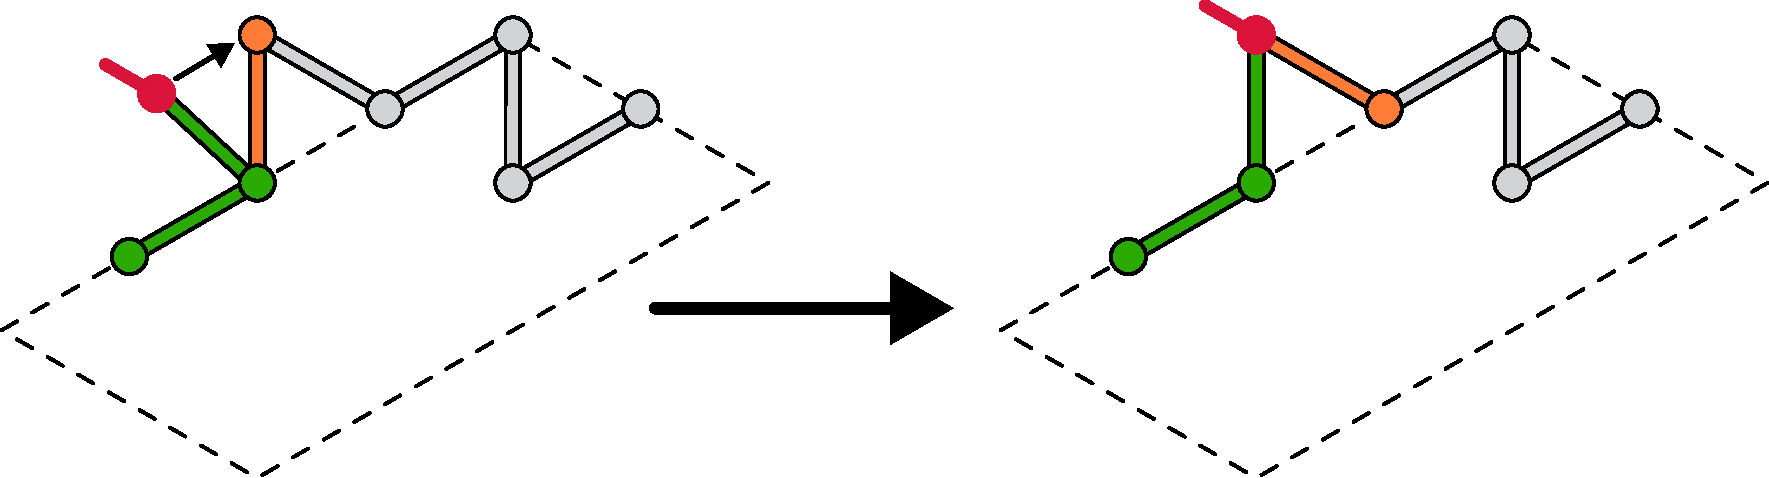
\includegraphics[width = 0.8\linewidth]{./implementation/figures/task-example.pdf}
\end{figureBox}

The participants have a timeout of 1 minute to complete the task. If they do not complete the task in the time limit, the task is marked as incomplete. The time each point is completed is recorded as well as the position of the hand and eye throughout the minute. The 5 different tasks are shown in Fig~\ref{fig:tasks} The participants are also given two demo tasks to get used to the system. \\

\begin{figureBox}[label={fig:tasks}, width=1.0\linewidth]{The 5 tasks}
    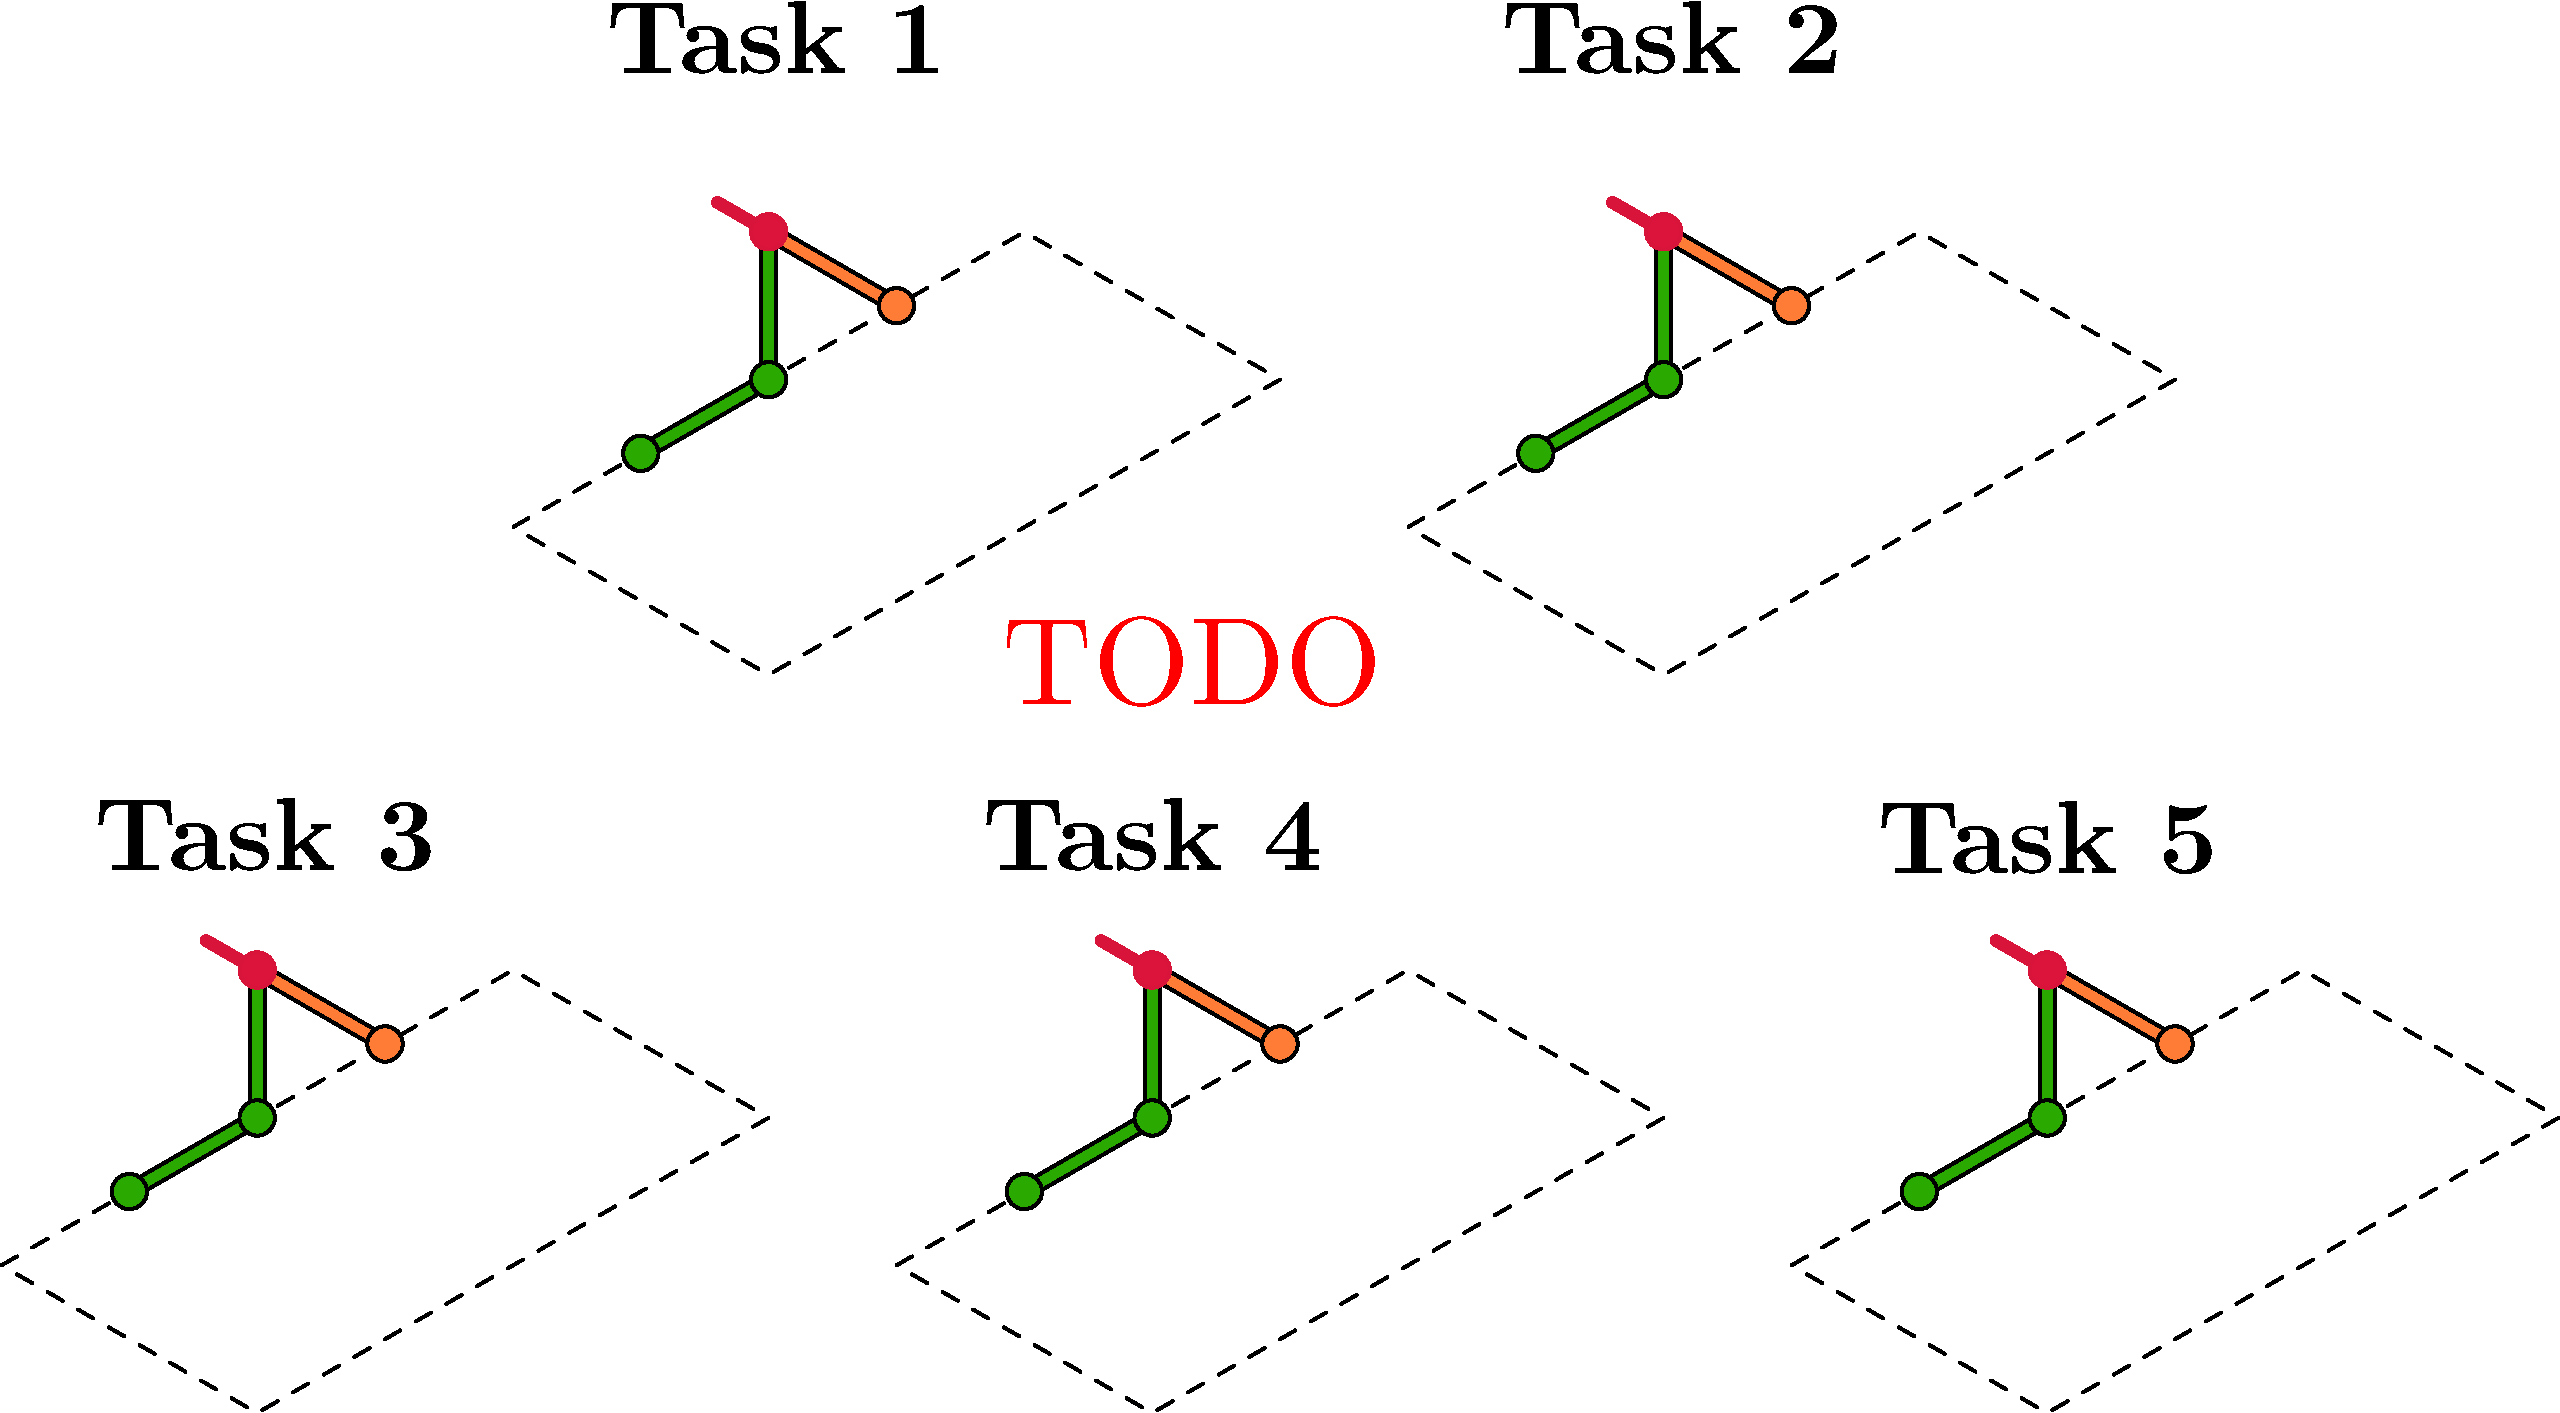
\includegraphics[width = 0.8\linewidth]{./implementation/figures/tasks.pdf}
\end{figureBox}

\subsection{Evaluation Metrics}
The evaluation metrics we used to evaluate the system were primarily the time taken to complete the task and the number of subtasks completed. We also recorded the eye and hand positions of the participants throughout the task.


\subsection{Participants}
We invited participant to take part in the study via email and text using a standardized script. On arrival the participants were asked to fill out a consent form and a questionnaire about themselves to find out information that might affect the results, such as their age, handedness and previous experience with VR/AR. \\   

They were next given a brief overview of the system and allowed to run through two demo tasks in different configurations to get used to the system. When they were comfortable with the system they were entered into our system and were automatically assigned a random order of the four conditions that can be seen in Fig~\ref{fig:study-conditions}. 

\begin{figureBox}[label={fig:study-conditions}, width=0.8\linewidth]{Study Conditions}
    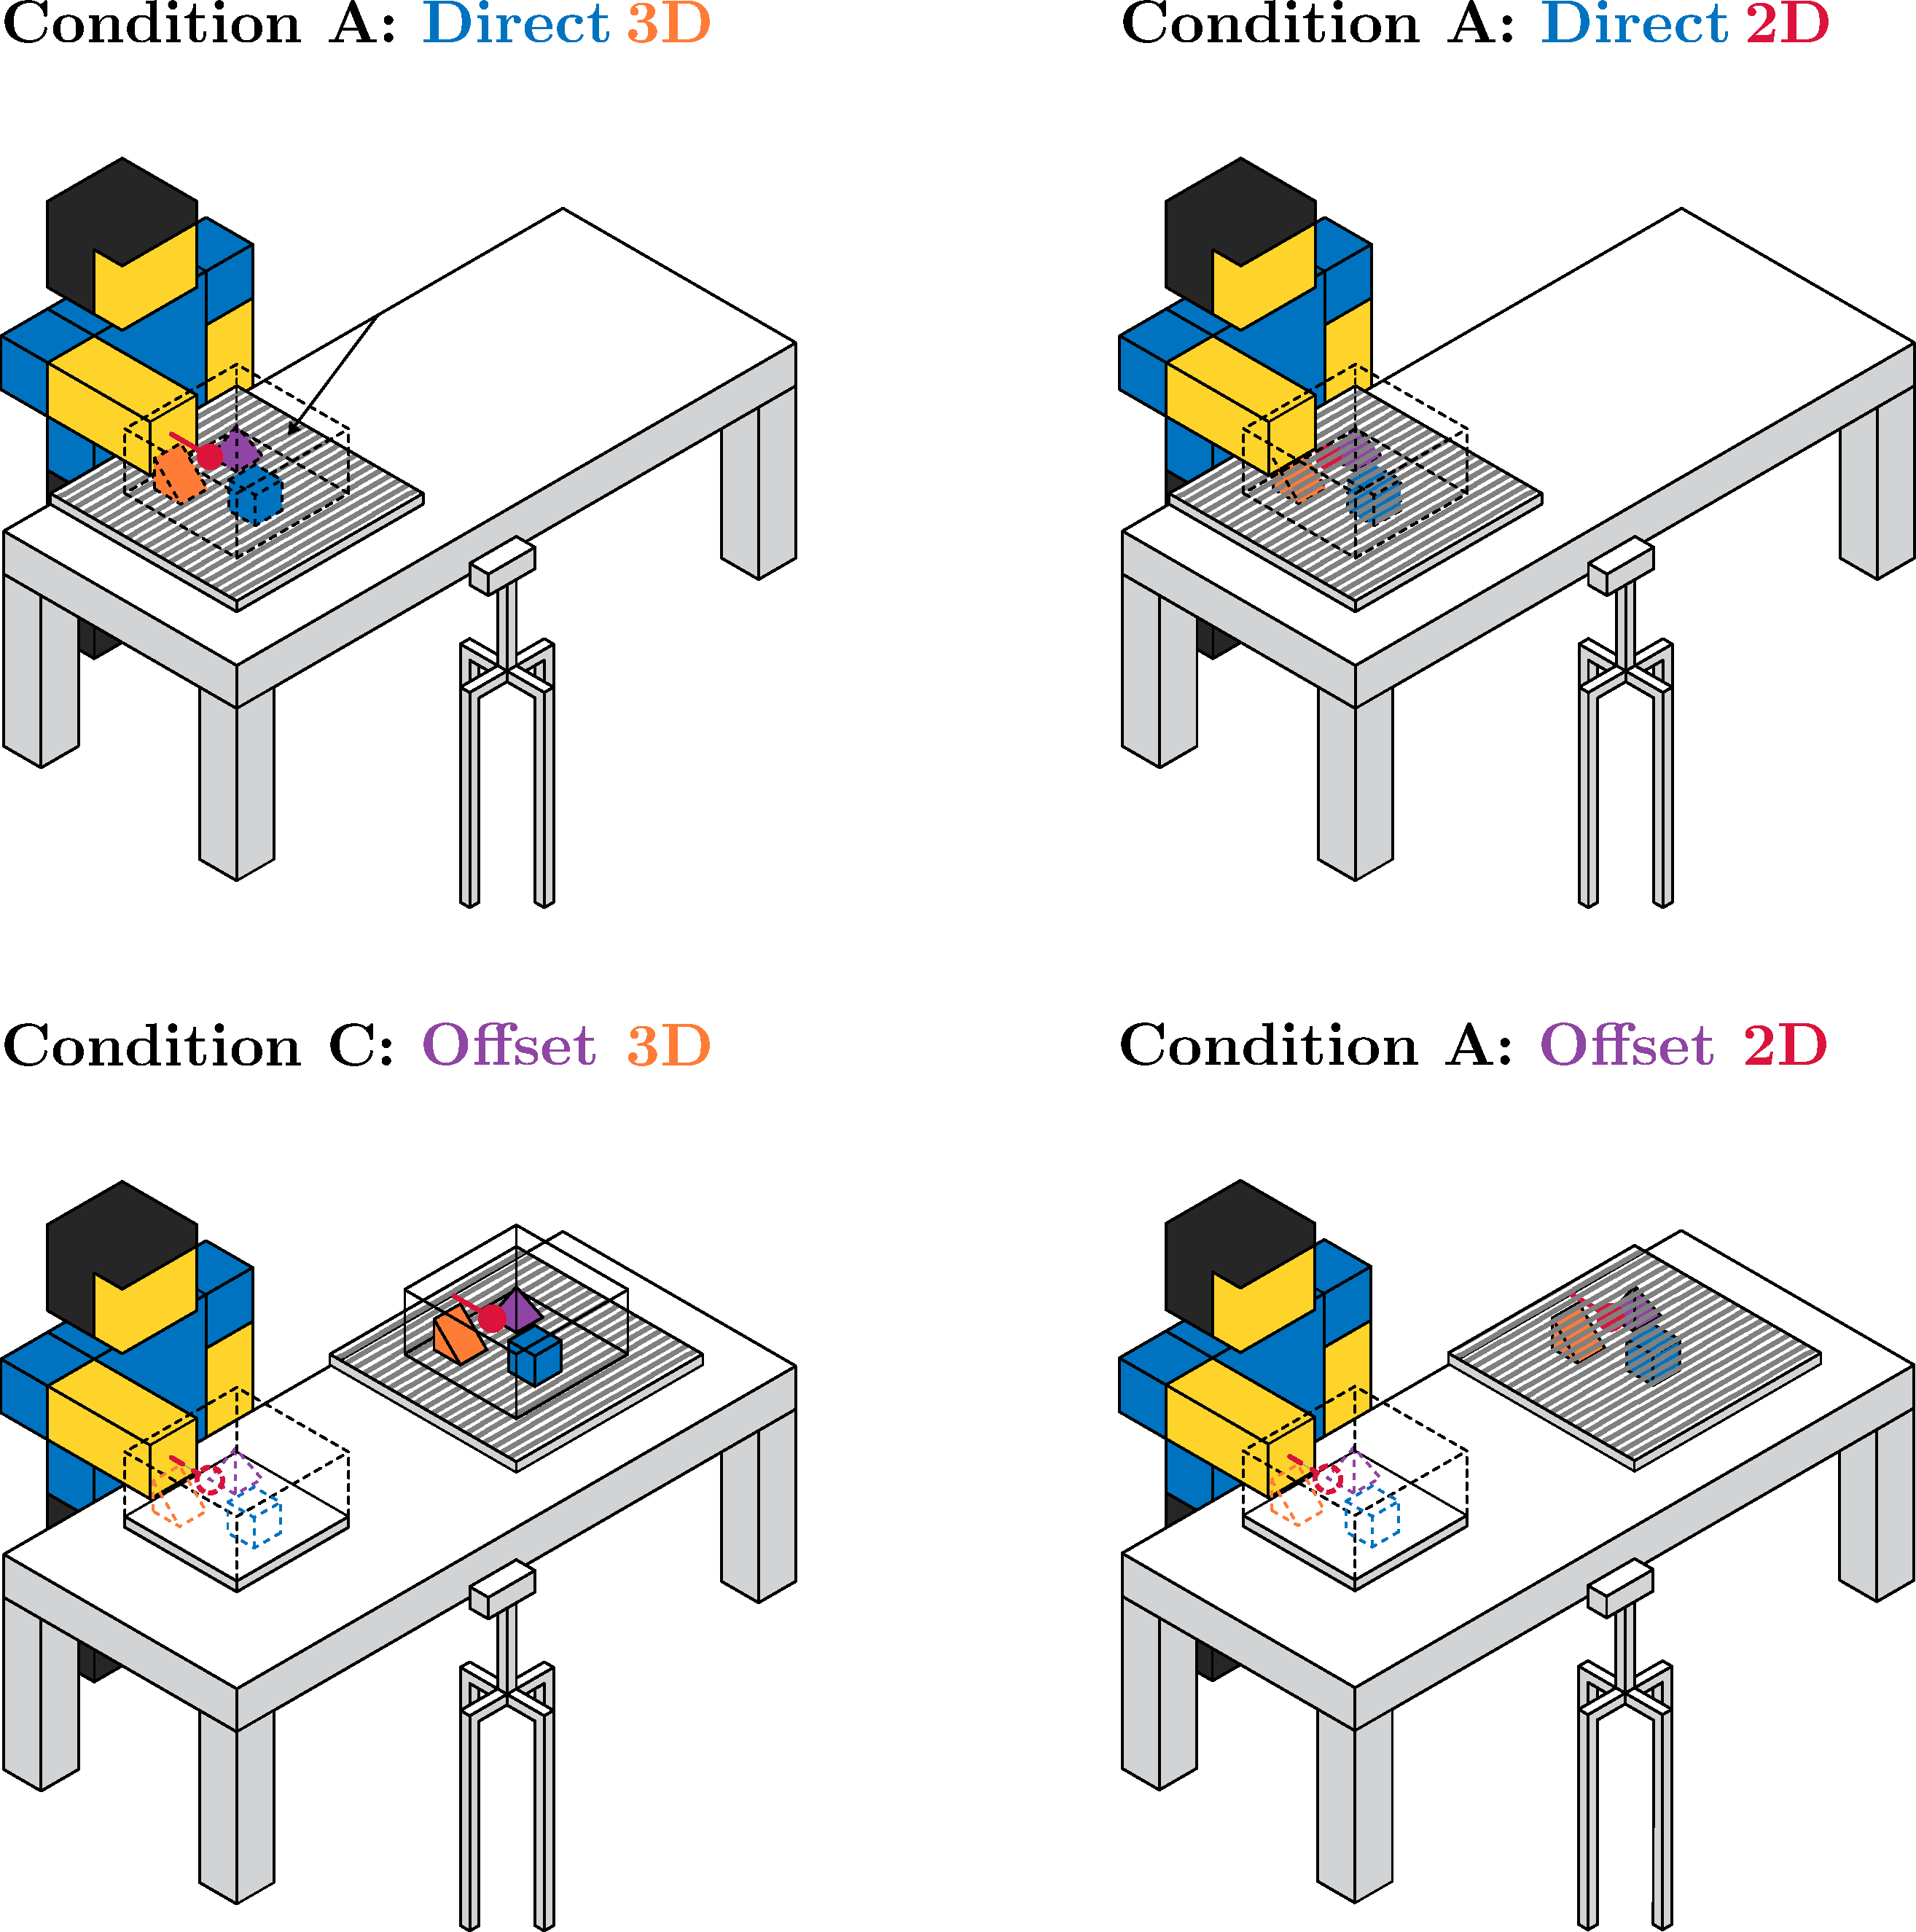
\includegraphics[width = 0.8\linewidth]{./implementation/figures/study-conditions.pdf}
\end{figureBox}

Each condition consisted of the 5, 1 minute tasks that the participants had to complete in order. The participants were allowed to take breaks between conditions. After each condition they were asked to fill out a survey about the condition. At the end of the study they were asked to fill out a survey about the system as a whole. The study was run in the Huxley building in Room 218 at Imperial College London.

\subsection{Study Implementation}

The study was run from a python based CLI using the Click library. The simulator was compiled as a shared library and called from the python CLI using a C-FFI. The results and logs were received from python in json format and stored in a mongoDB database. We then used this data to generate the results.

\textcolor{red}{if have time include code CLI snippet}

\subsection{Study Results}
\begin{enumerate}
	\item Use ANOVA test?
	\item ????
\end{enumerate}

\textcolor{red}{Do this once I've completed the study}